\documentclass[main.tex]{subfiles}

\begin{document}

\section{A3 Git: Branching}
Sie wollen Ihre Hello-World-Anwendung aus Aufgabe A2 um ein neues Feature zur Ausgabe von
»Goodbye Moon!« ergänzen. Erzeugen Sie dazu eine neue Klasse in einer neuen Datei. Nutzen
Sie den Feature Branch Workflow aus der Vorlesung und dokumentieren Sie zentrale Schritte
durch Screenshots (eine Iteration des Workflows genügt). Achten Sie dabei auf eine angemessene
Namensgebung, wie sie in der Vorlesung empfohlen wurde.

\subsection{Lösung 3}
\begin{figure}[H]
    \makebox[\textwidth][c]{
        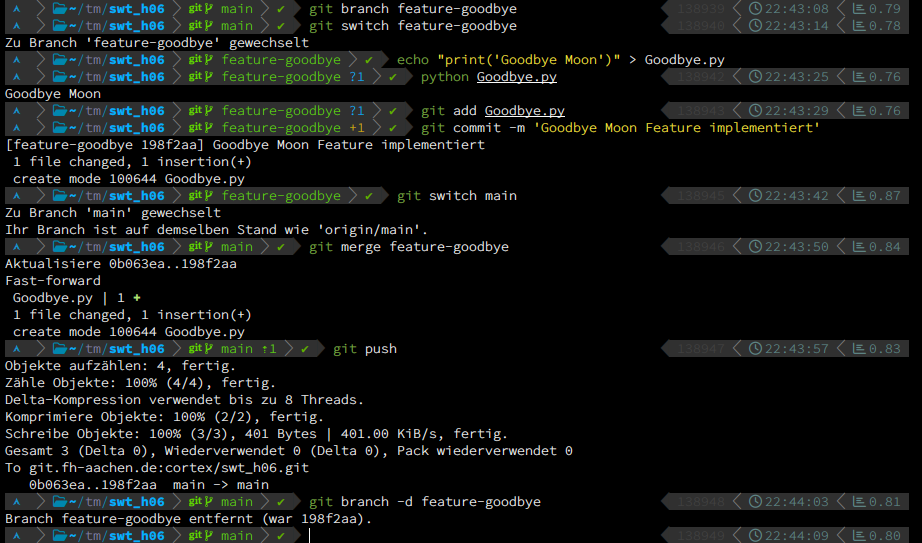
\includegraphics[width=1.2\linewidth]{s7.png}
    }
    \caption{Aufgabe 3}
    \label{fig:a1}
\end{figure}

\end{document}
